\documentclass[11pt]{article}
\usepackage[a4paper,margin=1in]{geometry}

\usepackage[T1]{fontenc}
\usepackage[utf8]{inputenc}
\usepackage{lmodern}
\usepackage{amsmath,amssymb}
\usepackage{booktabs}
\usepackage{array}
\usepackage{longtable}
\usepackage{graphicx}
\usepackage{tikz}
\usetikzlibrary{arrows.meta,positioning,fit,backgrounds,calc}
\usepackage{hyperref}
\hypersetup{
  colorlinks=true,
  linkcolor=black,
  citecolor=black,
  urlcolor=blue,
  pdftitle={ReproBot -- Second Progress Report},
  pdfauthor={Aleyna Kutuk, Engincan Varan, Gul Korkut, Goktug Mert Ozdogan}
}
\usepackage{xcolor}
\usepackage{caption}
\usepackage{pifont}

\definecolor{builtc}{HTML}{1B6F50}
\definecolor{missingc}{HTML}{97303F}
\definecolor{loopc}{HTML}{0E6E78}
\definecolor{warnc}{HTML}{97590C}

\newcommand{\built}{\textcolor{builtc}{\ding{51}}}
\newcommand{\absent}{\textcolor{missingc}{\ding{55}}}

\title{\textbf{ReproBot: A Multi-Agent System for Automated Scientific Paper Replication}\\[0.4em]
\large Second Progress Report}
\author{
  Aleyna Kütük \\ \small\texttt{aleynakutuk10@gmail.com}
  \and
  Engincan Varan \\ \small\texttt{engincanvaran@gmail.com}
  \and
  Gül Korkut \\ \small\texttt{serifegulkorkut@gmail.com}
  \and
  Göktuğ Mert Özdoğan \\ \small\texttt{goekmeroz@gmail.com}
}
\date{inzva AI Projects \#10 \\ 22.08.2026}


\begin{document}

\maketitle

\begin{abstract}
The first progress report described ReproBot as a proposed four-agent pipeline for
automated machine learning paper replication, supported by a literature review, an
implementation-ready project plan, and an early Reader prototype. This report covers the
implementation phase. Five of the seven planned components are now built and verified by
execution: PDF extraction, a five-field structured Reader, a Coder that emits a
self-contained training script, a Docker-sandboxed Runner, and an Orchestrator owning the
shared-memory state and the Coder\,$\leftrightarrow$\,Runner retry loop. Two papers --
\emph{Network In Network} and \emph{Wide Residual Networks} -- have been carried end to
end, from PDF through to a training script executing inside a container and reporting
metrics back. We report three substantive findings. First, the retry loop repairs real
defects: a deliberately reintroduced runtime fault was triaged, fed back to the Coder as
targeted feedback, and repaired on the first retry. Second, structured architecture
extraction measurably outranks the language model's pretrained priors -- given
\emph{Network In Network}, whose contribution is a custom \texttt{mlpconv} layer with no
memorized reference implementation, the Coder produced the correct layer cascade and
global-average-pooling head rather than the generic convolutional stack its priors would
favour. Third, several failure modes in LLM tool use are silent by construction and
require deterministic guards rather than prompt engineering. We are explicit about what
remains: the Critic does not exist, so no reproduced number has yet been compared against
any paper's claim, and the measured CPU throughput places a full-fidelity training run at
roughly 22 days per paper, making GPU access a precondition for any fidelity result.
\end{abstract}

\section{Introduction}
\label{sec:intro}

The first progress report \cite{reprobot2026first} established ReproBot's motivation and
design. The problem it addresses is unchanged: reproducing a machine learning paper's
empirical results is a mechanical task in principle and a labor-intensive one in
practice, and the large majority of published work ships no usable implementation --
across ICLR, ICML and NeurIPS 2024, only 16.7--21.2\% of accepted papers included a
working one \cite{seo2025papercoder}. The gap ReproBot targets is equally unchanged: no
surveyed system combines parsing a paper's claims, executing a faithful implementation,
and explicitly verifying the reproduced numbers against the published ones with a repair
loop driven by that comparison.

What has changed is that the system now exists in code. This report is therefore
structured around evidence rather than intent. Section~\ref{sec:architecture} describes
the architecture as implemented, and where it departs from the plan.
Section~\ref{sec:stages} documents each stage. Section~\ref{sec:results} reports the
measured results of running two papers through the full pipeline.
Section~\ref{sec:findings} collects engineering findings that we believe generalize
beyond this project. Section~\ref{sec:limitations} states the limitations plainly,
including the ones that prevent us from making any replication-fidelity claim at all.
Sections~\ref{sec:next} and \ref{sec:conclusion} cover next steps and conclusions.

Since the first report, the project has produced 30 commits across five newly implemented
pipeline stages totalling approximately 6{,}700 lines of Python, together with 21 logged
delegations to specialized coding, research, review and validation subagents.


\section{Positioning}
\label{sec:related}

The first report surveyed nine agentic-ML and paper-replication systems in detail. We do
not repeat that survey; instead we record where this phase's implementation choices
followed those precedents, where they diverged, and what the divergences cost or bought.

\textbf{Following AutoReproduce on execution feedback.} AutoReproduce's ablation is the
strongest available evidence that executing generated code matters more than inspecting
it: removing the debug-and-refine loop moved an LLM-judged alignment score only slightly
while nearly tripling the performance-gap metric \cite{zhao2025autoreproduce}. We took
this as decisive when sequencing the work, building the Runner and the execution-error
loop before the Critic, and Section~\ref{sec:results} reports a local instance of exactly
the phenomenon that ablation predicts.

\textbf{Diverging from AutoReproduce on edit granularity.} That system applies
line-range edits rather than regenerating a file, which reduces token cost and limits
collateral damage. Our Coder regenerates the whole script on every retry. This was a
deliberate simplification for a single-file target, and Section~\ref{sec:limitations}
records its cost: a successful repair can introduce a new defect elsewhere, and nothing
compares the semantics of successive attempts.

\textbf{Diverging from AutoP2C on repair scope.} AutoP2C localizes a fault to a file
before correcting it, machinery that exists because it targets a multi-file repository
\cite{lin2025autop2c}. Our Coder emits one self-contained script, so localization has
nothing to range over; the triage step supplies the diagnosis that localization would
otherwise provide.

\textbf{Retaining the tolerance gate as the differentiator.} Neither system compares a
reproduced number against the paper's claim under an explicit numeric tolerance. That
comparison remains ReproBot's distinguishing feature, and it remains unimplemented
(Section~\ref{sec:limitations}) --- a fact we would rather state than obscure.

\section{Implemented Architecture}
\label{sec:architecture}


\begin{figure}[tbp]
\centering
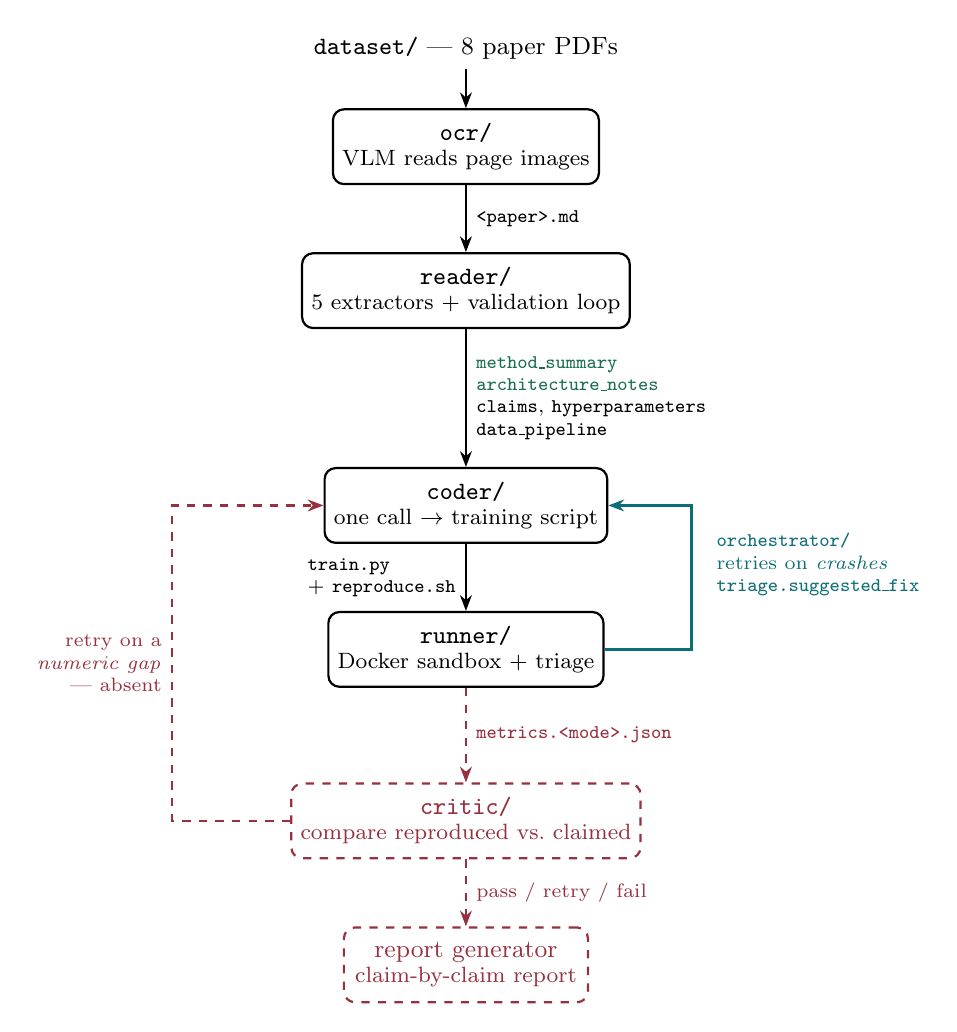
\begin{tikzpicture}[
  node distance=0.85cm and 1.5cm,
  stage/.style={draw, rounded corners, minimum width=3.1cm, minimum height=0.95cm,
    align=center, font=\small, thick},
  gone/.style={draw, rounded corners, minimum width=3.1cm, minimum height=0.95cm,
    align=center, font=\small, dashed, thick, draw=missingc, text=missingc},
  arr/.style={-{Stealth[length=2mm]}, thick},
  gonearr/.style={-{Stealth[length=2mm]}, thick, dashed, draw=missingc},
  looparr/.style={-{Stealth[length=2mm]}, very thick, draw=loopc},
  lbl/.style={font=\scriptsize, align=left},
  gonelbl/.style={font=\scriptsize, align=left, text=missingc}
]
  \node[stage] (ocr)    {\texttt{ocr/}\\[-2pt]\footnotesize VLM reads page images};
  \node[stage, below=of ocr] (reader) {\texttt{reader/}\\[-2pt]\footnotesize 5 extractors + validation loop};
  \node[stage, below=1.75cm of reader] (coder) {\texttt{coder/}\\[-2pt]\footnotesize one call $\to$ training script};
  \node[stage, below=of coder] (runner) {\texttt{runner/}\\[-2pt]\footnotesize Docker sandbox + triage};
  \node[gone,  below=1.2cm of runner] (critic) {\texttt{critic/}\\[-2pt]\footnotesize compare reproduced vs.\ claimed};
  \node[gone,  below=of critic] (report) {report generator\\[-2pt]\footnotesize claim-by-claim report};

  \node[above=0.5cm of ocr, font=\small] (pdf) {\texttt{dataset/} --- 8 paper PDFs};

  \draw[arr] (pdf) -- (ocr);
  \draw[arr] (ocr) -- node[right, lbl] {\texttt{<paper>.md}} (reader);
  \draw[arr] (reader) -- node[right, lbl]
    {\textcolor{builtc}{\texttt{method\_summary}}\\
     \textcolor{builtc}{\texttt{architecture\_notes}}\\
     \texttt{claims}, \texttt{hyperparameters}\\ \texttt{data\_pipeline}} (coder);
  \draw[arr] (coder) -- node[left, lbl] {\texttt{train.py}\\ + \texttt{reproduce.sh}} (runner);
  \draw[gonearr] (runner) -- node[right, gonelbl] {\texttt{metrics.<mode>.json}} (critic);
  \draw[gonearr] (critic) -- node[right, gonelbl] {pass / retry / fail} (report);

  % the real loop
  \draw[looparr] (runner.east) -- ++(1.1,0) |- (coder.east);
  \node[lbl, text=loopc, right=1.25cm of coder.east, anchor=west, yshift=-0.75cm]
    {\textbf{\texttt{orchestrator/}}\\ retries on \emph{crashes}\\ \texttt{triage.suggested\_fix}};

  % the absent loop
  \draw[gonearr] (critic.west) -- ++(-1.5,0) |- node[pos=0.25, left, gonelbl, align=right]
    {retry on a\\ \emph{numeric gap}\\ --- absent} (coder.west);
\end{tikzpicture}
\caption{ReproBot as implemented. Solid components are built and verified by execution;
dashed components in red do not exist. Two loops are shown and only one is real: the
Orchestrator retries on execution failures, routing the Runner's triage back to the Coder
as feedback. The absent loop --- retrying on a numeric gap between the reproduced value
and the paper's claim --- is the one the literature review identifies as missing from
every surveyed system, and it is missing here too.}
\label{fig:pipeline}
\end{figure}


The pipeline follows the planned Reader\,$\to$\,Coder\,$\to$\,Runner shape, with two
departures worth stating.

\textbf{The Reader emits five fields, not four.} The project plan specified
\texttt{method\_summary}, \texttt{claims}, \texttt{hyperparameters} and
\texttt{architecture\_notes}. All four are implemented. A fifth,
\texttt{data\_pipeline}, was added on the plan's own recommendation: data-processing
detail is the single weakest-covered aspect of paper-to-code extraction across every
surveyed system (56\% coverage in PaperCoder against 79--92\% elsewhere
\cite{seo2025papercoder}), and is therefore treated as a first-class output field rather
than folded into the method summary.

\textbf{The Runner's interface is a generated shell script, not a command line.} The
Coder emits a \texttt{reproduce.sh} alongside every training script, exposing four modes
--- \texttt{probe}, \texttt{smoke}, \texttt{capped} and \texttt{full} --- and the Runner
invokes nothing else. It never constructs a Python command and never passes a flag. This
keeps the Runner paper-agnostic: a future paper whose script requires entirely different
arguments changes only its own \texttt{reproduce.sh}. The contract narrows from eight
exactly-spelled command-line flags to four mode names.

The Orchestrator is implemented as a bounded, deterministic Python loop rather than the
LangGraph state machine the plan proposed. At the present scope the graph would comprise
three nodes and one conditional edge, which does not justify the dependency. The
shared-memory object follows the plan's schema exactly and the transition logic is
isolated in pure functions, so migration remains mechanical once the Critic introduces
genuine branching.


\subsection{The shared-memory object}

The Orchestrator owns one versioned object per paper, following the project plan's schema.
It is the artifact that lets the loop answer ``have we already tried this'' and that a
future Report Generator will read without re-deriving anything.

\begin{table}[htbp]
\centering
\small
\caption{The shared-memory object as implemented. \built{} denotes a field populated
today; \absent{} a field present in the schema but not yet written by any stage.}
\label{tab:state}
\begin{tabular}{llp{0.44\linewidth}}
\toprule
Field & & Contents \\
\midrule
\texttt{paper\_id}          & \built & Stem of the source paper \\
\texttt{reader\_output}     & \built & All five extraction fields, embedded \\
\texttt{coder\_output}      & \built & Script path, version, diff from previous attempt \\
\texttt{runner\_output}     & \built & Status, reproduced metrics, log paths, error trace \\
\texttt{critic\_output}     & \absent & Permanently \texttt{null}; reserved so the schema
                                        does not change when the Critic lands \\
\texttt{retry\_count}       & \built & Retries consumed \\
\texttt{retry\_budget}      & \built & Ceiling, default 2 \\
\texttt{history}            & \built & Append-only log of every stage transition, with
                                        timestamps \\
\texttt{attempts}           & \built & Per-attempt record: version, feedback given, runner
                                        status, triage category, plateau ratio \\
\bottomrule
\end{tabular}
\end{table}

Every attempt's script is archived beside the state file, so a run's full history is
reconstructable after the fact rather than only summarized.

\section{Stage Implementations}
\label{sec:stages}

\subsection{Extraction: \texttt{ocr/}}

Four independent PDF-to-Markdown backends share one command-line shape. The
vision-language backend renders each page to an image and sends it to Claude, so figures
are genuinely read rather than inferred from surrounding text --- a property the Reader's
architecture extraction depends on directly (Section~\ref{sec:reader}). Six of the eight
target papers are extracted. Two fail on a deterministic content-filter false positive,
diagnosed as originating in the vision classifier rather than in our prompt: the same
page fails identically at different render scales and under a minimal one-line prompt.

\subsection{Structured extraction: \texttt{reader/}}
\label{sec:reader}

Five extractors implement a shared abstract base class, so the pipeline treats every
stage uniformly and a new extraction type requires one new class and one line in the
stage list. A validator makes one further model call over the combined output and the
paper text, flagging inconsistencies without fixing them; the pipeline routes each flag
back to the single stage its \texttt{relates\_to} prefix names, re-runs that stage with
the flag folded into its prompt as feedback, and re-validates, capped at three passes.



\begin{figure}[tbp]
\centering
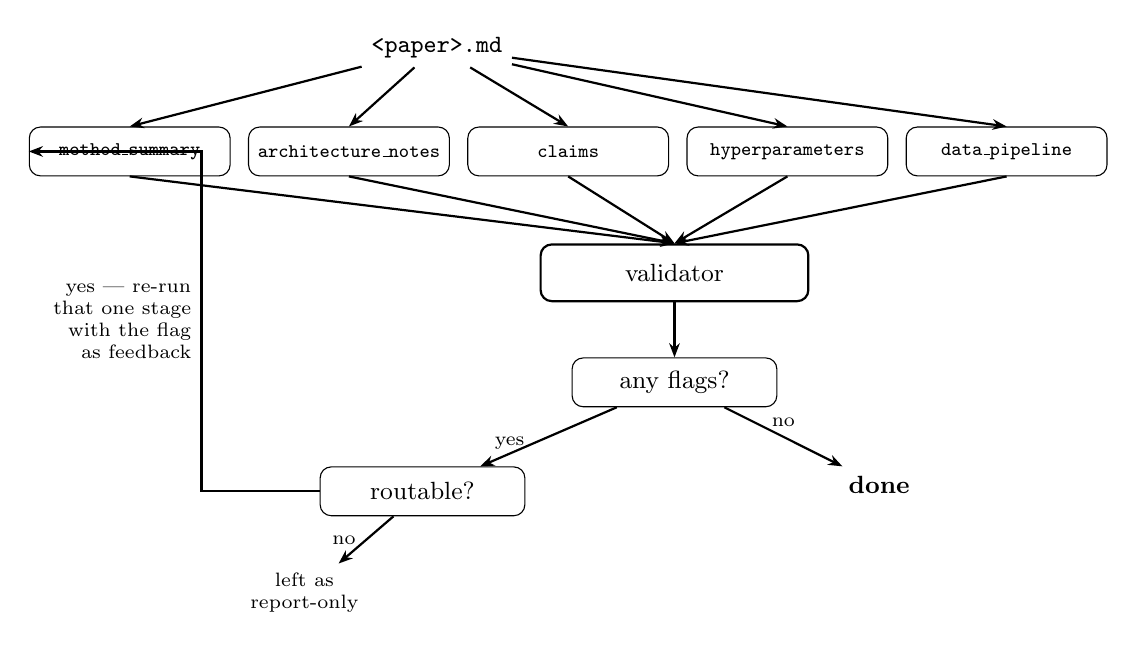
\begin{tikzpicture}[
  ex/.style={draw, rounded corners, minimum width=2.55cm, minimum height=0.62cm,
    align=center, font=\scriptsize\ttfamily},
  val/.style={draw, rounded corners, minimum width=3.4cm, minimum height=0.72cm,
    align=center, font=\small, thick},
  dec/.style={draw, rounded corners, minimum width=2.6cm, minimum height=0.62cm,
    align=center, font=\small},
  arr/.style={-{Stealth[length=1.8mm]}, thick},
  lbl/.style={font=\scriptsize, align=left}
]
  \node[font=\small] (md) {\texttt{<paper>.md}};
  \node[ex, below=0.75cm of md, xshift=-3.9cm] (e1) {method\_summary};
  \node[ex, right=0.22cm of e1] (e2) {architecture\_notes};
  \node[ex, right=0.22cm of e2] (e3) {claims};
  \node[ex, right=0.22cm of e3] (e4) {hyperparameters};
  \node[ex, right=0.22cm of e4] (e5) {data\_pipeline};

  \node[val, below=0.85cm of e3, xshift=1.35cm] (v) {validator};
  \node[dec, below=0.7cm of v] (q) {any flags?};
  \node[dec, below=0.75cm of q, xshift=-3.2cm] (route) {routable?};
  \node[font=\small, below=0.75cm of q, xshift=2.6cm] (done) {\textbf{done}};
  \node[lbl, below=0.6cm of route, xshift=-1.5cm, align=center] (report)
    {left as\\ report-only};

  \draw[arr] (md) -- (e1.north);
  \draw[arr] (md) -- (e2.north);
  \draw[arr] (md) -- (e3.north);
  \draw[arr] (md) -- (e4.north);
  \draw[arr] (md) -- (e5.north);

  \foreach \n in {e1,e2,e3,e4,e5} { \draw[arr] (\n.south) -- (v.north); }

  \draw[arr] (v) -- (q);
  \draw[arr] (q) -- node[above, lbl] {no} (done);
  \draw[arr] (q) -- node[left, lbl, pos=0.6] {yes} (route);
  \draw[arr] (route) -- node[left, lbl] {no} (report);
  \draw[arr] (route.west) -- ++(-1.5,0) |- node[pos=0.25, left, lbl, align=right]
    {yes --- re-run\\ that one stage\\ with the flag\\ as feedback} (e1.west);
\end{tikzpicture}
\caption{The Reader's five extractors and its validation retry loop. All five read the
same Markdown and none consumes another's output, so they are independent and the order is
only reading order. The validator sees the paper text plus all five results and flags
rather than fixes. A flag whose \texttt{relates\_to} prefix names exactly one stage is
routed back to it; a flag spanning two stages is left as report-only, because attributing
a genuine cross-stage disagreement to one side is not a solved problem. The loop is capped
at three validation passes.}
\label{fig:reader}
\end{figure}


\subsubsection{The five extractors}

Each extractor is a class implementing a shared abstract base: a name, and an
\texttt{extract} method taking the paper's Markdown, a client, and an optional feedback
string. The uniformity is what makes the retry loop stage-agnostic --- it calls
\texttt{extract}, keys results by name, and on a validation flag routes it back to
whichever stage owns that name. Adding \texttt{data\_pipeline}, then
\texttt{method\_summary} and \texttt{architecture\_notes}, each required one new class and
one line in the stage list, with no change to the loop, the validator, or the routing.

\begin{table}[htbp]
\centering
\small
\caption{The Reader's five extraction stages and their consumers.}
\label{tab:extractors}
\begin{tabular}{lp{0.36\linewidth}p{0.28\linewidth}}
\toprule
Stage & Extracts & Consumed by \\
\midrule
\texttt{method\_summary}     & Problem, core idea, novelty, prose summary & Coder context;
                                                                            Report Generator \\
\texttt{architecture\_notes} & Components, equations, scaling rule, unstated details &
                                                                            Coder (primary) \\
\texttt{claims}              & Metric, dataset, value, unit, source, variant & Critic
                                                                            (future) \\
\texttt{hyperparameters}     & Name, value as string, unit, source, variant & Coder \\
\texttt{data\_pipeline}      & Per-dataset preprocessing, augmentation, splits; reference
                               URLs & Coder \\
\bottomrule
\end{tabular}
\end{table}

Two schema decisions recur across stages and are worth stating once. Values that could be
numbers are kept as \emph{strings} --- a learning-rate schedule reading ``0.1 initial,
dropped by 0.2 at epochs 60, 120 and 160'' must survive verbatim rather than collapsing to
a scalar, and ``not stated'' must remain expressible. And every extracted item carries a
\texttt{source} naming the table, figure block, or prose section it came from, with a
transcribed page number, so a downstream consumer or a human can check it.

\subsubsection{The validation retry loop}

After all five stages run, a validator makes one further call over the paper text and the
combined output. It is prompted to \emph{flag}, not fix, two classes of problem:
inconsistencies between stages, and content in the paper that looks like it should have
been captured and was not. Each flag carries a \texttt{relates\_to} field.

The loop then routes. A flag whose prefix matches exactly one stage name is sent back to
that stage, which re-runs with the flag's text folded into its prompt --- a full
re-extraction addressing a specific complaint, not a patch to individual fields. A flag
that does not map to exactly one stage, such as a cross-check between two of them, is
left in the output as report-only and never auto-retried, because attributing a genuine
cross-stage disagreement to one side is not a solved problem.

A worked example from an early run against \emph{Wide Residual Networks}: the first pass
extracted 73 claims, and the validator caught that one of them labelled a 4.00\% value as
a CIFAR-100 result when it was the paper's CIFAR-10 value from the same table row,
duplicated under the wrong dataset label. The claims stage re-ran with that complaint and
the misattributed entry was removed. This is the loop working as designed, and it is a
defect that no schema constraint would have caught.

\subsubsection{Recording what the paper does not say}

The \texttt{architecture\_notes} stage carries a required \texttt{unstated\_details} list.
Its rationale differs from the rest of the pipeline's ``do not guess'' discipline in one
respect that we think is worth drawing out.

Elsewhere, recording ``not stated'' is simply honest. Here it is load-bearing, because the
consumer is a code generator and code has to run. An extractor that invents a plausible
channel count does not produce an obvious error --- it produces a model that trains
successfully and reports a number for the \emph{wrong network}. The failure is silent and
the artifact looks correct. Making the gap explicit moves the decision downstream, where
the Coder must choose a value and disclose that it chose it.

For \emph{Network In Network} the stage records twelve such gaps, quoting the paper's own
deferral --- ``the detailed settings of the parameters are provided in the supplementary
materials'' --- rather than supplying the values from elsewhere.

\subsubsection{Distinguishing the paper's own equations from its contrasts}

A paper introducing a new layer typically prints the conventional formulation, and often a
rival's, beside its own. \emph{Network In Network} prints all three within two pages: the
conventional convolution it replaces, its own \texttt{mlpconv} computation, and maxout's,
which it argues against.

Returned as an undifferentiated list of LaTeX strings, these are three plausible
specifications, and a code generator will implement one of them. Instructing the model to
omit the baselines did not work --- it continued to return them, which is unsurprising,
since they are genuinely relevant context for understanding the method. Requiring the
\emph{schema} to carry an \texttt{is\_own\_method} flag on every entry did work
immediately, and the classification proved correct across all four papers processed
(Table~\ref{tab:reader}).

The distinction survives into the generated code: the Coder implements only entries marked
as the paper's own, and Section~\ref{sec:results} confirms that it did.

\subsubsection{Shared guards for tool use}

All six model calls in the Reader route through one module holding the request and its
response guards, rather than each stage parsing responses itself. This consolidation was
prompted by the failure modes in Section~\ref{sec:findings}, and it means a fix lands once
rather than six times. It also makes the failure reporting uniform: a guard names the
stage that misbehaved, the keys it expected, and the keys it actually received.

\subsection{Code generation: \texttt{coder/}}

One model call converts a paper's Reader output plus its Markdown into a self-contained
HuggingFace \texttt{Trainer} script. The stage never executes what it writes and never
imports a deep-learning framework: it calls the model and writes files, leaving execution
entirely to the Runner. Three things determine what it produces --- how its inputs are
ranked, what is checked before a script is accepted, and the interface it emits alongside
the script.


\subsubsection{Input precedence}

The Coder receives two documents: the paper's Reader output and the paper's Markdown. Its
prompt ranks them explicitly, and adds a third rank that is not a document at all.

\begin{enumerate}
  \item \texttt{architecture\_notes}, \texttt{hyperparameters} and \texttt{data\_pipeline}
        --- validated, source-grounded, and authoritative wherever they carry a value.
  \item The paper's Markdown --- corroboration, and the source for anything the extraction
        does not cover.
  \item The model's own recollection of a well-known architecture --- last resort, and
        usable only when disclosed in the output's \texttt{assumptions} field.
\end{enumerate}

The third rank is unusual enough to justify. A code generator cannot decline to produce a
value the way an extractor can: something must be written where a channel count goes. The
ranking therefore does not forbid using prior knowledge, which would be unenforceable, but
requires that its use be visible. Section~\ref{sec:results} reports what that looks like
in practice.

\subsubsection{Two deterministic gates}

Before a generated script is accepted, two checks run. Neither involves a model call and
neither costs anything.

The script must parse as valid Python; a failure writes the source to a separate path for
inspection and marks the run failed, rather than emitting broken code. And every
command-line flag the Runner depends on must literally appear in the script's text, with
the model's own claim about which flags it defined cross-checked against that text, since
a model can report a flag it did not write.

The limits of both gates are discussed in Section~\ref{sec:findings}: parsing establishes
that a script is syntactically well-formed, never that it runs.

\subsubsection{The generated interface}

Alongside every training script the Coder emits a \texttt{reproduce.sh} whose four modes
are the Runner's entire vocabulary (Table~\ref{tab:modes}). The header of that file
doubles as an audit trail, listing the targeted claim, every hyperparameter with the paper
value behind it, and every assumption the Coder had to make.

\begin{table}[htbp]
\centering
\small
\caption{The four modes of the generated \texttt{reproduce.sh}. Each writes its own
metrics file, so a cheap stage's numbers cannot be mistaken for a real run's.}
\label{tab:modes}
\begin{tabular}{lll}
\toprule
Mode & Cost & What it establishes \\
\midrule
\texttt{probe}  & 2 optimizer steps      & Data $\to$ model $\to$ loss $\to$ step works;
                                           catches shape and dtype errors \\
\texttt{smoke}  & 1 epoch, small slice   & Execution reaches evaluation and the metrics
                                           write \\
\texttt{capped} & 5 epochs, 512 images   & Training learns --- accuracy climbs above
                                           chance \\
\texttt{full}   & The paper's own setup  & The only numbers comparable to the claim;
                                           requires a GPU \\
\bottomrule
\end{tabular}
\end{table}

Passing \texttt{full} supplies no flags at all, because every default in the generated
script is already the paper's own value. The cheaper modes are overrides.

\subsection{Sandboxed execution: \texttt{runner/}}

The Runner executes a generated script inside a container, escalating through the modes of
Table~\ref{tab:modes} and stopping at the first failure. Three aspects proved less
straightforward than expected --- how the image is built and mounted, how a wall-clock
budget is actually enforced on a container, and how a failure is classified --- and are
treated in turn below.


\subsubsection{Container design}

The image is built from a slim Python base with CPU-only PyTorch installed from the
dedicated index, rather than from a vendor image carrying CUDA layers that a CIFAR-scale
CPU run never touches. The result is 1.69\,GB and builds in approximately 224\,s.

No generated code is copied into the image. The paper's output directory is bind-mounted
at run time, which keeps the image static across regenerations --- the Coder can rewrite
every script in the project without invalidating a layer --- and is also how results
return: the script writes its metrics file into the mounted directory, which is the host
directory, so no copy step is required.

A shared dataset cache is mounted alongside. Its value is measurable: the same
\texttt{probe} stage takes 1774\,s against a cold cache and 166\,s against a warm one,
nearly all of the difference being a one-time 170\,MB download that all eight target
papers would otherwise repeat.

\subsubsection{The timeout trap}

Enforcing a wall-clock budget on a container is less direct than it appears, and the
obvious implementation is wrong. Terminating the client process that launched the
container does not stop the container: it is a child of the daemon, not of the launching
process, and it continues running, holding its mounts and consuming CPU.

Every run is therefore launched with an explicit name chosen in advance --- after the
client dies, that name is the only remaining handle --- and on expiry the container is
killed by name, treating an already-reaped container as success. A second subtlety: the
timeout exception carries whatever partial output it had collected as raw bytes even when
the call was made in text mode, so decoding must be defensive or the handler reporting the
timeout crashes while doing so.

Budgets are per-stage and enforced independently, so a hung cheap stage cannot consume the
budget of the expensive one behind it. They are calibrated against a measured run rather
than estimated: an earlier estimate would have timed out on the first cold-cache execution,
producing a failure indistinguishable from a hung script.

\subsubsection{Triage}

A failed run is classified by a single cheap model call into a defect in the generated
script or a problem with the environment. Success and timeout are classified mechanically
with no model call at all --- the exit status already answers the question, and inviting a
judgment where none is needed costs money on the common path and adds a way to be wrong.

The classification is not merely descriptive: it determines routing
(Section~\ref{sec:orchestrator}). Logs are captured in full to disk and separately
truncated for the model's prompt, retaining both the head, where import and setup failures
appear, and the tail, where the traceback is.

\subsection{The retry loop: \texttt{orchestrator/}}

The Orchestrator owns the shared-memory object and the loop. Its routing order is
deliberate: an environmental error stops immediately rather than consuming retries,
because regenerating a script cannot repair a broken container. A timeout likewise stops,
since no triage is produced for timeouts by design and a slow but correct script must not
be ``repaired'' into a different one. Only a recoverable error regenerates.

A plateau guard compares each regenerated script against its predecessor and stops early
when they are near-identical, rather than exhausting the budget on a fix that is not
changing anything --- following PaperBench's observation that agents plateau rather than
making steady long-horizon progress \cite{starace2025paperbench}.


\subsubsection{Verdicts}
\label{sec:orchestrator}

The loop terminates in one of seven verdicts (Table~\ref{tab:verdicts}). Three are
success or benign stops; four are failures distinguished by what a retry could possibly
achieve.

\begin{table}[htbp]
\centering
\small
\caption{Terminal verdicts. Only \texttt{recoverable} failures within budget produce
another attempt.}
\label{tab:verdicts}
\begin{tabular}{lp{0.55\linewidth}}
\toprule
Verdict & Meaning \\
\midrule
\texttt{success}                & A stage passed; nothing to retry \\
\texttt{environment\_error}     & The container or its inputs are at fault; regenerating
                                  the script would change nothing \\
\texttt{timeout}                & Exceeded the wall-clock budget; no triage is produced,
                                  and a slow but correct script must not be rewritten \\
\texttt{retry\_budget\_exhausted} & Recoverable, but out of attempts \\
\texttt{plateaued}              & The regenerated script was near-identical to the one
                                  that just failed \\
\texttt{untriaged\_error}       & Failed with no triage available to route on \\
\texttt{coder\_failed}          & Generation itself failed, e.g.\ the syntax gate \\
\bottomrule
\end{tabular}
\end{table}

The check order matters and is fixed. An environmental error is tested \emph{before} the
retry budget, because consuming a retry on a broken container wastes an attempt on a fault
the Coder cannot address. A timeout stops for a different reason: no triage exists to
route on, and a script that is slow but correct must not be ``repaired'' into a different
one.

\subsubsection{The plateau guard}

Before spending a container run on a regenerated script, the Orchestrator compares it
line-wise against its predecessor and stops early if they are near-identical, rather than
exhausting the budget on a fix that is not changing anything. This follows PaperBench's
observation that agents plateau rather than making steady long-horizon progress
\cite{starace2025paperbench}.

One implementation detail proved to matter more than expected. The standard sequence
matcher applies a heuristic that discards frequently repeated elements, which on source
code discards common lines. Measured on the same pair of scripts, the heuristic reported a
similarity of 0.9975 while the exact comparison reported 0.7625 --- against a 0.98
threshold, the difference between stopping and continuing. The heuristic is disabled, and
the measured ratio is logged on every retry so the threshold can be tuned from data rather
than remaining a guess.


\begin{figure}[tbp]
\centering
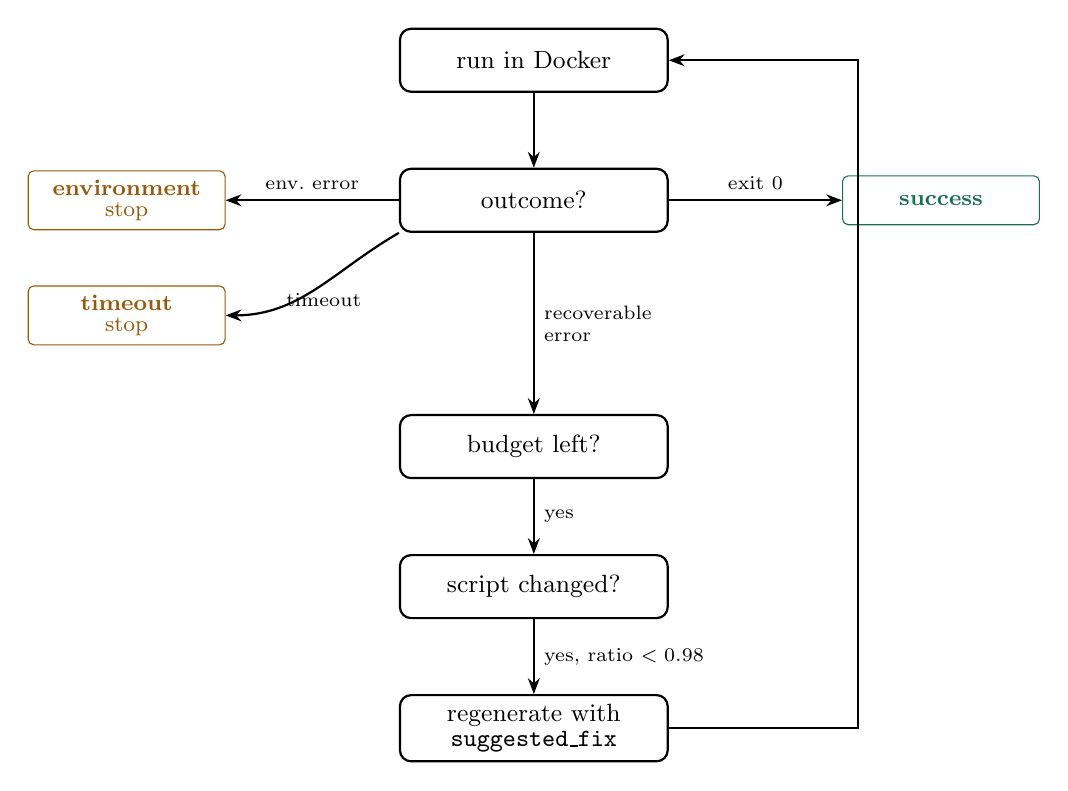
\begin{tikzpicture}[
  dec/.style={draw, rounded corners, minimum width=3.4cm, minimum height=0.8cm,
    align=center, font=\small, thick},
  term/.style={draw, rounded corners=2pt, minimum width=2.5cm, minimum height=0.62cm,
    align=center, font=\footnotesize},
  arr/.style={-{Stealth[length=2mm]}, thick},
  lbl/.style={font=\scriptsize}
]
  \node[dec] (run) {run in Docker};
  \node[dec, below=0.95cm of run] (status) {outcome?};
  \node[dec, below=2.3cm of status] (budget) {budget left?};
  \node[dec, below=0.95cm of budget] (plateau) {script changed?};
  \node[dec, below=0.95cm of plateau] (regen) {regenerate with\\[-2pt]\texttt{suggested\_fix}};

  \node[term, right=2.2cm of status, draw=builtc, text=builtc] (ok) {\textbf{success}};
  \node[term, left=2.2cm of status, draw=warnc, text=warnc] (env) {\textbf{environment}\\[-2pt]stop};
  \node[term, below=0.7cm of env, draw=warnc, text=warnc] (to) {\textbf{timeout}\\[-2pt]stop};

  \draw[arr] (run) -- (status);
  \draw[arr] (status) -- node[above, lbl] {exit 0} (ok);
  \draw[arr] (status) -- node[above, lbl] {env.\ error} (env);
  \draw[arr] (status.south west) to[out=210, in=0] node[below, lbl, pos=0.45] {timeout} (to.east);
  \draw[arr] (status) -- node[right, lbl, align=left] {recoverable\\ error} (budget);
  \draw[arr] (budget) -- node[right, lbl] {yes} (plateau);
  \draw[arr] (plateau) -- node[right, lbl] {yes, ratio $<0.98$} (regen);
  \draw[arr] (regen.east) -- ++(2.4,0) |- (run.east);
\end{tikzpicture}
\caption{The Orchestrator's routing. The order is deliberate: an environmental error stops
\emph{before} the retry budget is consulted, because regenerating a script cannot repair a
broken container. A timeout also stops rather than retrying --- no triage is produced for
timeouts by design, and a slow but correct script must not be ``repaired'' into a
different one. Only a recoverable error, within budget, whose regenerated script actually
differs from its predecessor, results in another execution.}
\label{fig:loop}
\end{figure}


\section{Results}
\label{sec:results}

\subsection{Extraction coverage}

Table~\ref{tab:reader} reports the Reader's output across the four papers processed. The
\emph{own/eq} column is the most informative: it counts equations marked as the paper's
own against the total captured. \emph{All Convolutional Net} prints six equations of
which two are its own; \emph{Wide Residual Networks} prints one and it is its own. A
field that always returned every equation would be useless to a code generator.

\begin{table}[htbp]
\centering
\small
\caption{Reader output across four papers. \emph{Comp.} is architecture components;
\emph{own/eq} is own-method equations over equations captured; \emph{Gaps} is
\texttt{unstated\_details} entries; \emph{Flags} is unresolved validation flags after the
three-pass cap.}
\label{tab:reader}
\begin{tabular}{lrrrrcrr}
\toprule
Paper & Claims & Hyp. & Data & Comp. & own/eq & Gaps & Flags \\
\midrule
Network In Network      & 12 & 17 & 4 &  7 & 1/3 & 12 & 4 \\
All Convolutional Net   & 17 & 13 & 4 & 10 & 2/6 & 11 & 5 \\
Deep Residual Learning  & 66 & 28 & 6 & 10 & 2/3 &  7 & 8 \\
Wide Residual Networks  & 61 & 20 & 4 & 11 & 1/1 & 11 & 6 \\
\bottomrule
\end{tabular}
\end{table}

Validation does not converge. Every paper finishes with flags remaining after the cap,
and the count is worst on the paper with the most claims. Inspection shows a substantial
proportion are the validator raising a concern and dismissing it within its own
description rather than identifying a real defect. We regard this as a genuine limitation
of the current design rather than a tuning problem, and record it as such.

\subsection{End-to-end execution}

Both papers with generated scripts were carried through the Orchestrator. Both succeeded
on the first attempt with no retries required (Table~\ref{tab:runs}).

\begin{table}[htbp]
\centering
\small
\caption{End-to-end runs. Both papers reached \texttt{smoke} and returned
\texttt{success} with zero retries consumed. Reproduced values are reported to
demonstrate that the measurement path works end to end; they are \emph{not}
replication results (Section~\ref{sec:limitations}).}
\label{tab:runs}
\begin{tabular}{lrrrr}
\toprule
Paper & probe & smoke & Reproduced & Claimed \\
\midrule
Network In Network     &  32.2\,s &  62.1\,s & 86.72\% & 10.41\% \\
Wide Residual Networks & 241.4\,s & 367.2\,s & 89.45\% &  4.00\% \\
\bottomrule
\end{tabular}
\end{table}

The roughly sixfold difference in wall clock reflects model size: WRN-28-10 carries
approximately 36.5M parameters against \emph{Network In Network}'s order of 1M. The
reproduced error rates are far from the claimed values, and this is the expected and
correct behaviour of the stages that produced them --- \texttt{probe} and \texttt{smoke}
train for one epoch over a few hundred images and exist to answer whether the script
runs, never whether the number is right.

\subsection{The retry loop repairs real defects}

The loop was validated against a deliberately reintroduced fault: a learning-rate
scheduler whose method reads an attribute its constructor never assigns. The fault is
valid Python, so the syntax gate admits it, and it raises only when the training loop
first logs the learning rate. This is precisely the class of defect the loop exists for.

The container run failed with an \texttt{AttributeError}; triage classified it as
recoverable and produced a targeted fix naming the class and the missing assignment; the
Coder regenerated with that text folded into its prompt; the plateau guard measured a
similarity of 0.41 against the previous attempt, well below the 0.98 stopping threshold;
and the second attempt passed. The repair was not incidental --- the regenerated script
retained the class the triage named and added exactly the missing assignment.

This is the local counterpart of AutoReproduce's ablation, in which removing the
debug loop barely moved an LLM-judged alignment score while nearly tripling the
performance-gap metric \cite{zhao2025autoreproduce}: code can read as a faithful
implementation and still be wrong if it is never executed.

\subsection{Architecture extraction outranks pretrained priors}

The Coder was verified against \emph{Network In Network} rather than \emph{Wide Residual
Networks}, deliberately. A wide residual network is among the most thoroughly memorized
architectures in the literature and would be reproduced correctly from priors alone,
demonstrating nothing about the extraction. \emph{Network In Network} is the honest test:
its \texttt{mlpconv} layer is the paper's contribution, its dimensions appear nowhere in
the paper, and its equation list contains two decoys.

The generated script contains a genuine \texttt{mlpconv} cascade --- a $k\times k$
convolution followed by two $1\times1$ convolutions, with a docstring mapping each line
to the paper's Equation~2 --- and contains no fully-connected layer at all, retaining the
global-average-pooling classifier that is the paper's second contribution. Both decoy
equations are explicitly excluded and named as excluded.

The strongest evidence is negative. A priors-driven implementation of this paper is a
plain convolutional stack with a fully-connected head; both of those defaults were
avoided, and the generated script justifies the avoidance by citing components tagged
\texttt{[baseline, not own method]} --- a label from our extraction schema, not language
from the paper.

We qualify this in one respect. The channel widths in the generated model are the
canonical configuration, drawn from the model's own knowledge rather than from the paper,
which genuinely omits them. This is the designed outcome and it is disclosed in the
output. The change made those values \emph{visible} rather than \emph{correct}, and a
Critic will need to weight a disclosed prior below a paper-sourced value.


\subsection{Cost}

A Reader pass over one paper issues six model calls --- five extractions and one
validation --- and each retry round adds one call per flagged stage plus one further
validation. Observed runs use twelve to fourteen calls per paper against the three-pass
cap. The Coder adds one call per generation attempt, and the Runner one cheap
classification per genuine failure, which is zero on a clean run.

Two design choices hold this down. Triage is not invoked on success or timeout, so the
common path costs nothing beyond generation. And the deterministic gates --- syntax,
required flags, plateau similarity --- catch what they can without a model call at all.

The dominant cost is not the model but the compute, and it is not close: at the measured
throughput, one full-fidelity training run exceeds the entire project's model spend to
date by orders of magnitude in wall-clock terms alone.

\section{Engineering Findings}
\label{sec:findings}

\subsection{Silent failure modes in structured tool use}

Three distinct failure modes were observed in which a model call returns a structurally
valid response that is nonetheless empty or wrong, in a way indistinguishable from a
correct extraction over a paper that had nothing to report.

The first is output truncation at the token limit, which yields a partial payload.
The second is an intermittent well-formed response with every required field absent.
The third is the most instructive: a \emph{double-encoded} payload, in which the model
returns a clean tool-use response whose single key holds the entire result re-encoded as
a JSON string. Field lookups then all miss and the extraction is discarded. It reproduced
three times out of three on one paper, and fired again during later verification, where
without the guard it would have reported zero datasets on an apparently clean run.

All three are now handled in one shared module rather than at six call sites. The general
lesson is that structured-output failures do not necessarily announce themselves as
errors, and a pipeline that treats a well-formed empty response as a legitimate negative
result will silently accumulate them.

\subsection{Schemas constrain models more reliably than instructions}

Two independent cases: instructing the model to omit baseline equations did not stop it
returning them, whereas requiring a per-entry \texttt{is\_own\_method} flag produced
correct classification immediately; and a bookkeeping field the model never populated,
despite being schema-required on every run, was eliminated by deriving it from data
already present rather than by asking more insistently. Where a value is computable from
what has already been extracted, computing it is more reliable than requesting it.

\subsection{Static gates cannot establish that generated code runs}

Two defects reached generated scripts that passed every deterministic gate. The first is
the scheduler fault described above. The second, found by inspection, is a divergence
between a script's own bookkeeping --- which describes one stage as $192\to192\to10$ ---
and the code it emitted, which builds $192\to10\to10$. The script runs, and the choice is
a defensible reading of a dimension the paper never states; what is wrong is that the
record describes a different network from the code.

Neither is reachable by parsing. Both argue for the execution-driven loop rather than for
additional static analysis.

\subsection{Platform constraints shaped the architecture}

The development machine is an Intel Mac, and no PyTorch release supports both Python 3.13
and Intel macOS: 3.13 support arrived in the same release range that dropped Intel-macOS
wheels. Reducing to Python 3.11 installs PyTorch 2.2.2, but current \texttt{transformers}
requires 2.5 or newer and, on finding an older version, silently disables its PyTorch
backend rather than raising.

This is why the Runner executes inside a container rather than on the host. The container
runs its own Linux Python, so the constraint does not apply within it, and the project's
dependency lock stays free of PyTorch entirely.


\section{Development Methodology}
\label{sec:methodology}

This phase was built through a delegation pattern that we record because it shaped the
result, and because two of its failures are instructive.

Work was decomposed into scoped tasks dispatched to specialized subagents --- research
agents that survey precedent and propose a design without writing code, coding agents that
implement a scoped change and verify it by running it, review agents that critique an
artifact before a costly or hard-to-repeat action, and validation agents that audit
existing output read-only. Each delegation, its brief, and its outcome is logged; 21 are
recorded for this phase.

Two failures are worth reporting honestly, because both were caught only by independent
verification rather than by the reports themselves.

In one case, a coding agent's report asserted it had left four modules untouched; the
version control diff showed all four had been refactored. The refactor was an improvement
--- it consolidated guards that had been duplicated --- but the discrepancy meant the
agent's verification claims could not be relied upon, and the affected pipeline was re-run
directly. In another, an agent predicted a specific failure by reading a ``known issues''
section and mistaking a historical, already-discarded defect for current state; the claim
was false and a single search of the source disproved it.

The generalizable lesson is narrow but practical: an agent's description of its own change
is a claim about the world, and the cost of checking it against the repository is close to
zero. We now treat the diff, not the report, as the record of what happened.

\section{Limitations}
\label{sec:limitations}

We state these directly, because several bear on how the results above should be read.

\textbf{No fidelity claim is possible yet.} The Critic does not exist. Nothing in the
system compares a reproduced number against a paper's claim, and the field reserved for
that verdict is permanently null. The reproduced error rates in Table~\ref{tab:runs}
demonstrate that the measurement path works; they are not replication results and should
not be read as any.

\textbf{Full-fidelity runs are not currently feasible.} Measured throughput is 5.256
training samples per second for WRN-28-10 on this CPU. The paper's setup is 50{,}000
samples over 200 epochs, placing one paper and one claim at approximately 22 days. Every
result reported here comes from stages that train for one epoch over a few hundred
images. GPU access is a precondition for any fidelity measurement, not an optimization.

\textbf{The evidence base is two papers.} Both succeeded on the first attempt, so the
retry loop's behaviour in production remains demonstrated only by the injected fault.
Four of the loop's seven terminal verdicts have been exercised only against test doubles.

\textbf{Retries regenerate rather than patch.} A repair rewrites the whole file, so a
successful fix can introduce a new defect elsewhere, and nothing compares the semantics of
successive attempts. AutoReproduce's line-range edit mechanism
\cite{zhao2025autoreproduce} is the natural remedy and is not yet implemented.

\textbf{Validation does not converge}, as reported in Section~\ref{sec:results}, and two
of the eight target papers cannot currently be extracted at all.

\section{Next Steps}
\label{sec:next}

\textbf{The Critic} is the highest-value remaining component and closes the loop the
project's thesis rests on. Its verdict logic should remain simple, auditable arithmetic
against an explicit numeric tolerance rather than a model judging numbers by eye ---
Agent Laboratory's automated reviewer overestimated quality by 2.3 points against human
judges \cite{schmidgall2025agentlab}, and an objective numeric check is precisely the
failure mode ReproBot exists to avoid. It can be built and tested against synthetic
metrics immediately; its verdicts become meaningful when compute allows a real run.

\textbf{GPU compute} should be secured in parallel rather than afterwards, since it gates
every fidelity result.

\textbf{Coverage} should be extended across the remaining papers, which requires no new
code and would convert single demonstrations into distributions.

\textbf{The Report Generator} is the promised deliverable and the cheapest remaining
component: the shared-memory object already carries everything it needs, including the
append-only history log.

\section{Conclusion}
\label{sec:conclusion}

ReproBot has moved from design to a working pipeline. Five of seven components are
implemented and verified by execution; two papers have been carried from PDF to a
training script running in a sandbox; the retry loop repairs real defects; and structured
architecture extraction demonstrably outranks the language model's priors on a paper
where those priors would otherwise dominate.

What has been demonstrated is that the machinery works end to end. What has not been
demonstrated --- and cannot be, until the Critic exists and compute allows a full training
run --- is replication fidelity, which is the project's actual claim. We regard stating
that distinction clearly as more useful than reporting an aggregate that would obscure it.

\bibliographystyle{plain}
\begin{thebibliography}{9}

\bibitem{reprobot2026first}
Kütük, A., Varan, E., Korkut, G., \& Özdoğan, G.~M. (2026).
ReproBot: A Multi-Agent System for Automated Scientific Paper Replication --- First
Progress Report. \textit{inzva AI Projects \#10}.

\bibitem{starace2025paperbench}
Starace, G., Jaffe, O., Sherburn, D., Aung, J., et al. (2025).
PaperBench: Evaluating AI's Ability to Replicate AI Research.
\textit{arXiv:2504.01848}.

\bibitem{seo2025papercoder}
Seo, M., Baek, J., Lee, S., \& Hwang, S.~J. (2025).
Paper2Code: Automating Code Generation from Scientific Papers in Machine Learning.
\textit{arXiv:2504.17192}.

\bibitem{zhao2025autoreproduce}
Zhao, X., Sun, M., Wang, W., et al. (2025).
AutoReproduce: Automatic AI Experiment Reproduction with Paper Lineage.
\textit{arXiv:2505.20662}.

\bibitem{lin2025autop2c}
Lin, Z., Li, M., Chen, S., et al. (2025).
AutoP2C: An LLM-Based Agent Framework for Code Repository Generation from Multimodal
Content in Academic Papers. \textit{arXiv:2504.20115}.

\bibitem{schmidgall2025agentlab}
Schmidgall, S., Su, Y., Wang, Z., et al. (2025).
Agent Laboratory: Using LLM Agents as Research Assistants.
\textit{arXiv:2501.04227}.

\bibitem{li2024mlrcopilot}
Li, R., Patel, T., Wang, Q., \& Du, X. (2024).
MLR-Copilot: Autonomous Machine Learning Research based on Large Language Models Agents.
\textit{arXiv:2408.14033}.

\end{thebibliography}

\end{document}
